\section[Bagging et Forêts Aléatoires]{Bagging et Forêts Aléatoires}

\subsection[Introduction]{Introduction}

\begin{frame}{Motivation pour le Bagging}
	\begin{itemize}
		\item On a vu précédemment que CART peut entraîner du sur-apprentissage avec des réglages trop agressifs de ses hyper-paramètres (taille minimum de feuille, entropie minimum, profondeur maximum).
		\item \`A l'inverse, des réglages trop conservateurs peuvent conduire à du sous-apprentissage.
		\item Bien qu'il soit possible de régler ces paramètres afin d'obtenir un compromis satisfaisant, nous allons explorer une autre approche: le \textbf{bagging} (bootstrap aggregating).
		\item La combinaison de CART et du bagging donne naissance à un nouvel algorithme: \textbf{Les Forêts Aléatoires} !
	\end{itemize}
\end{frame}

\begin{frame}{Idée générale du Bagging}
	L'idée générale du Bagging peut se résumer dans les points suivants:
	\begin{itemize}
		\item On réalise $B$ ré-échantillonnages des données d'apprentissage en utilisant l'algorithme du bootstrapping.
		\pause
		\item Sur chaque échantillon on entraîne un arbre avec des réglages plutôt agressifs, quitte à introduire de la variance. On veut avant tout, limiter le biais.
		\pause
		\item Pour contre-balancer le risque de sur-apprentissage résultant de notre choix précédent, au moment de réaliser une prédiction, tous les arbres entraînés réalisent une prédiction et cette prédiction est \textbf{moyennée}.
		\pause
		\item Le Bagging fait partie des méthodes \textbf{ensemblistes} en apprentissage automatique.
	\end{itemize}
\end{frame}

\subsection[Algorithme]{Algorithme}

\begin{frame}{Particularité des Forêts Aléatoires}
	En plus du Bagging, les Forêts Aléatoires introduisent une subtilité supplémentaire. Dans l'algorithme CART, à l'étape multi-dimensionnelle, on n'explore plus \textbf{toutes} les caractéristiques d'entrée mais un \textbf{sous-ensemble aléatoire}:
	\begin{itemize}
		\item On remplace l'étape 1: Pour chaque $j \in \llbracket 1;d \rrbracket$ on applique l'algorithme mono-dimensionnel en considérant la caractéristique $X_j$.
		\item Par:
		\begin{enumerate}
			\item On détermine le nombre de caractéristiques à considérer, en général $d^* = \lfloor \sqrt{d} \rfloor$.
			\item On sélectionne aléatoirement les caractéristiques en réalisant $d^*$ tirages sans remise dans un ensemble constitué de toutes les caractéristiques $\{1, 2, \cdots d\}$.
		\end{enumerate}
	\end{itemize}
\end{frame}

\begin{frame}{Prise de décision}
	Pour une prédiction sur des données d'inférence $x_i$ on interroge les $B$ arbres créés et on effectue une moyenne. Si on note $P_k^{(b)}(x_i) \in [0, 1]$ la probabilité prédite par l'arbre $b$ pour la classe $k$ sur les données $x_i$, alors la prédiction réalisée par l'algorithme de Bagging est:
	\begin{equation*}
		P_k(x_i) = \frac{1}{B} \sum_{b=1}^B P_k^{(b)}(x_i)
	\end{equation*}
	C'est cette opération qui permet de réduire la variance introduite par chaque arbre dans la Forêt Aléatoire. Elle est appelée Soft voting.
\end{frame}


\subsection[Cas d'étude]{Cas d'étude}

\begin{frame}{Chiffres manuscrits MNIST}
	On prendra pour exemple le dataset MNIST, introduit dans le cours sur l'analyse en composantes principales, qui contient des images en niveaux de gris de chiffres écrits à la main: \href{https://www.kaggle.com/datasets/hojjatk/mnist-dataset}{\textbf{Kaggle MNIST Dataset}}.
	\begin{itemize}
		\item Yann LeCun, Courant Institute, NYU
		\item Corinna Cortes, Google Labs, New York
		\item Christopher J.C. Burges, Microsoft Research, Redmond
	\end{itemize}
\end{frame}

\begin{frame}{Simplification et algorithmes}
	Nous entraînerons une Forêt Aléatoire sur ces données MNIST en utilisant une simplification des données obtenue par analyse en composantes principales.

	\vspace{0.5cm}

	Les algorithmes de Scikit-Learn que nous utiliserons:
	\begin{itemize}
		\item \href{https://scikit-learn.org/stable/modules/generated/sklearn.decomposition.PCA.html}{\texttt{sklearn.decomposition.PCA}}
		\item \href{https://scikit-learn.org/stable/modules/generated/sklearn.tree.DecisionTreeClassifier.html}{\texttt{sklearn.tree.DecisionTreeClassifier}}
		\item \href{https://scikit-learn.org/stable/modules/generated/sklearn.ensemble.RandomForestClassifier.html}{\texttt{sklearn.ensemble.RandomForestClassifier}}
	\end{itemize}
\end{frame}

\begin{frame}{Classification multi-classes}
	Nous disposons à présent d'un problème de classification à classes multiples. Cela nécessite quelques ajustements aux métriques de performance que nous avons rencontrées:
	\begin{itemize}
		\item Matrice de confusion: $C$.
		\item Courbe ROC: $\mathcal{C}_{\text{ROC}}$.
		\item Surface sous la courbe ROC: $\operatorname{AUC}$.
	\end{itemize}
\end{frame}

\begin{frame}{Classification multi-classes: matrice de confusion}
	La définition que nous avions introduite au premier chapitre reste d'actualité:
	\begin{block}{Définition: Matrice de confusion}
		En classification à $K$ classes, la matrice de confusion $C \in \mathcal{M}_{K,K}$ est définie comme suit en fonction des classes \textbf{réelles} $y^{(i)}$ et des classes \textbf{prédites} $\hat{y}^{(i)}$ pour chaque observation $i$:
		\begin{equation}
			C_{m,n} = \operatorname{card} \left( \{i \in \{1, 2, \cdots, n\}\} \mid y^{(i)} = m \, \text{et} \, \hat{y}^{(i)} = n \right)
			\nonumber
		\end{equation}
	\end{block}
	\vspace{0.5cm}
	\pause
	La différence est que l'on ne peut plus associer directement aux éléments de la matrice $C$ les \textbf{vrais positifs}, \textbf{faux positifs}, \textbf{vrais négatifs} et \textbf{faux négatifs}.
\end{frame}

\begin{frame}{Classification multi-classes: stratégie One vs Rest}
	Une approche générale est de calculer ces taux $\operatorname{VP}$, $\operatorname{FP}$, $\operatorname{VN}$, $\operatorname{FN}$ pour chaque classe $k$ en utilisant une stratégie One vs Rest:
	
	\begin{equation*}
		\begin{aligned}
			\operatorname{VP}_k &= \operatorname{card} \left( \{i \in \{1, 2, \cdots, n\}\} \mid y^{(i)} = k \, \text{et} \, \hat{y}^{(i)} = k \right) \\
			\operatorname{FP}_k &= \operatorname{card} \left( \{i \in \{1, 2, \cdots, n\}\} \mid y^{(i)} \ne k \, \text{et} \, \hat{y}^{(i)} = k \right) \\
			\operatorname{VN}_k &= \operatorname{card} \left( \{i \in \{1, 2, \cdots, n\}\} \mid y^{(i)} \ne k \, \text{et} \, \hat{y}^{(i)} \ne k \right) \\
			\operatorname{FN}_k &= \operatorname{card} \left( \{i \in \{1, 2, \cdots, n\}\} \mid y^{(i)} = k \, \text{et} \, \hat{y}^{(i)} \ne k \right)
		\end{aligned}
	\end{equation*}
	
\end{frame}

\begin{frame}{Classification multi-classes: courbe ROC en stratégie One vs Rest}
	Avec ces nouvelles définitions on peut définir, pour la classe $k$, un taux des vrais positifs $\operatorname{TVP}_k$ et un taux des faux positifs $\operatorname{TFP}_k$:
	\begin{equation*}
		\begin{cases}
			\operatorname{TVP}_k = \displaystyle \frac{\operatorname{VP}_k}{\operatorname{VP}_k + \operatorname{FN}_k} \\[10pt]
			\operatorname{TFP}_k = \displaystyle \frac{\operatorname{FP}_k}{\operatorname{FP}_k + \operatorname{VN}_k}
		\end{cases}
		\nonumber
	\end{equation*}
	\pause
	Et proposer une définition pour la courbe ROC:
	\begin{block}{Définition: Courbe ROC One vs Rest}
		Pour une classe $k$, la courbe ROC, notée $\mathcal{C}_{\text{ROC},k}$ représente la relation entre le taux de vrais positifs $\operatorname{TVP}_k$ et le taux de faux positifs $\operatorname{TFP}_k$ quand le seuil de décision $\theta$ change:
		\begin{equation*}
			\mathcal{C}_{\text{ROC},k} = \{ \left(\operatorname{TFP}_k, \operatorname{TVP}_k\right) \in [0, 1]^2 \mid \theta \in [0, 1]\}
		\end{equation*}
	\end{block}
\end{frame}

\begin{frame}{Classification multi-classes: AUC en stratégie One vs Rest}
	Enfin, la surface sous la courbe ROC pour la classe $k$, que l'on notera $\operatorname{AUC}_k$ peut se définir en fonction du seuil de décision $\theta \in [0, 1]$ et $t \in [0, 1]$ du taux de faux positifs pour une valeur de $\theta$ donnée: $t = \operatorname{TFP}_k(\theta)$:
	\begin{block}{Définition: AUC One vs Rest}
		Pour une classe $k$, la surface sous la courbe ROC, notée $\operatorname{AUC}_k$ se définit comme:
		\begin{equation*}
			\operatorname{AUC}_k = \int_{t = 0}^{t = 1} \operatorname{TVP}_k(t) dt
		\end{equation*}
	\end{block}
\end{frame}

\begin{frame}{Exemples de résultats}
	Voici un résultat obtenu sur le dataset MNIST en utilisant une Forêt Aléatoire:
	\begin{columns}
		\begin{column}{0.5\textwidth}
			\begin{figure}
				\centering
				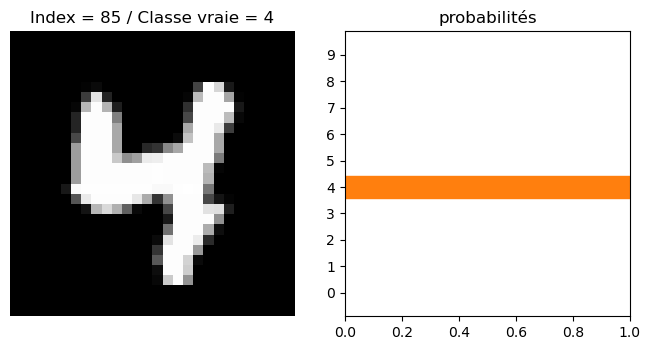
\includegraphics[width=1.0\linewidth]{Images/MNIST_1}
				\label{fig:MNIST_1}
			\end{figure}			
		\end{column}
		\begin{column}{0.5\textwidth}
			\begin{figure}
				\centering
				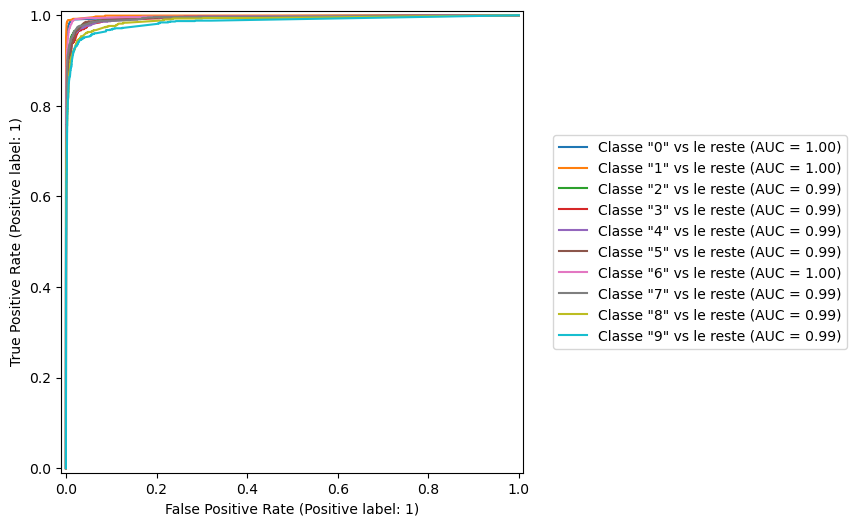
\includegraphics[width=1.0\linewidth]{Images/MNIST_2}
				\label{fig:MNIST_2}
			\end{figure}			
		\end{column}
	\end{columns}	
\end{frame}

\subsection[Synthèse]{Synthèse}

\begin{frame}{Forêts Aléatoires (Bagging)}
	\begin{figure}
		\centering
		\resizebox{0.95\textwidth}{!}{
			\begin{tikzpicture}[
				>=stealth,
				node distance=1.5cm and 2.5cm,
				data/.style={rectangle, rounded corners, draw=black, fill=blue!10, minimum width=2.5cm, minimum height=1cm, align=center},
				tree/.style={rectangle, draw=black, fill=green!15, minimum width=2.5cm, minimum height=1cm, align=center},
				agg/.style={rectangle, rounded corners, draw=black, fill=orange!20, minimum width=3cm, minimum height=1cm, align=center},
				arrow/.style={thick, ->}
				]
				
				% Noeuds
				\node[data] (D) {Données $\mathcal{D}$};
				\node[tree] (T2) [right=3cm of D] {Arbre 2\\(Profond)};
				\node[tree] (T1) [above=0.5cm of T2] {Arbre 1\\(Profond)};
				\node[tree] (T3) [below=0.5cm of T2] {Arbre $B$\\(Profond)};
				\node[agg] (Vote) [right=2cm of T2] {Moyenne\\(Soft voting)};
				\node (Out) [right=1.5cm of Vote] {\textbf{Prédiction}};
				
				% Fleches
				\draw[arrow] (D) -- node[above, sloped, midway, font=\footnotesize] {Bootstrap 1} (T1.west);
				\draw[arrow] (D) -- node[above, midway, font=\footnotesize] {Bootstrap 2} (T2.west);
				\draw[arrow] (D) -- node[below, sloped, midway, font=\footnotesize] {Bootstrap $B$} (T3.west);
				
				\draw[arrow] (T1.east) -- (Vote.west);
				\draw[arrow] (T2.east) -- (Vote.west);
				\draw[arrow] (T3.east) -- (Vote.west);
				
				\draw[arrow] (Vote) -- (Out);
				
				% Variables
				\node[text=green!40!black, font=\footnotesize, align=center] at (5.5, 2.5) {\textit{Sous-ensembles aléatoires}\\\textit{de $d^*$ caractéristiques}\\\textit{à chaque découpe}};
				
			\end{tikzpicture}
		}
	\end{figure}
	\vspace{0.5cm}
	Architecture \textbf{parallèle}. On réduit la \textbf{variance} d'arbres complexes et indépendants.
\end{frame}